%\VignetteIndexEntry{Glimma Vignette}
%\VignetteKeyword{RNA-Seq}
%\VignetteKeyword{differential expression}
%\VignetteKeyword{interactive graphics}
%\VignettePackage{Glimma}
%\usepackage[utf8]{inputenc}
\documentclass{article}

\RequirePackage{/usr/local/lib/R/site-library/BiocStyle/resources/tex/Bioconductor}

\AtBeginDocument{\bibliographystyle{/usr/local/lib/R/site-library/BiocStyle/resources/tex/unsrturl}}
\usepackage{hyperref}
\usepackage{graphicx}
\newcommand{\Rarg}[1]{\textcolor{BlueGreen}{{\sf{#1}}}}
\newcommand{\Rfun}[1]{\textcolor{VioletRed}{{\sf{#1}}}}

\usepackage{Sweave}
\begin{document}
\input{Glimma-concordance}

\title{Glimma: interactive graphics for differential expression analyses of RNA-seq data}
\author{Shian Su, Charity W. Law, Matthew E. Ritchie}
\date{First edition 28 January, 2016\\
Last revised \today}
\maketitle

\tableofcontents

\section{Quick start}\label{sec:quickstart}
\Biocpkg{Glimma} is a \Bioconductor{} package for interactive visualization of results from differential expression analyses of RNA-sequencing (RNA-seq) data. Its functionality is intended to enhance reporting capabilities so that such results can be explored more conveniently by end-users. Glimma, which loosely stands for interactive {\bf G}raphics from {\bf limma}, extends some of the popular plotting capabilities in the \Biocpkg{limma} \cite{limma} package such as multi-dimensional scaling (MDS) plots and mean-difference (MD) plots. Glimma is designed to handle objects native to limma, as well as from \Biocpkg{edgeR} \cite{edgeR} and \Biocpkg{DESeq2} \cite{DESeq2} packages, with its output as a html page containing interactive displays (Figure~\ref{fig:overview}).
Displays within Glimma were inspired by visualisations from {\it Degust} software \cite{Degust}.

\begin{figure}[!ht]
  \centerline{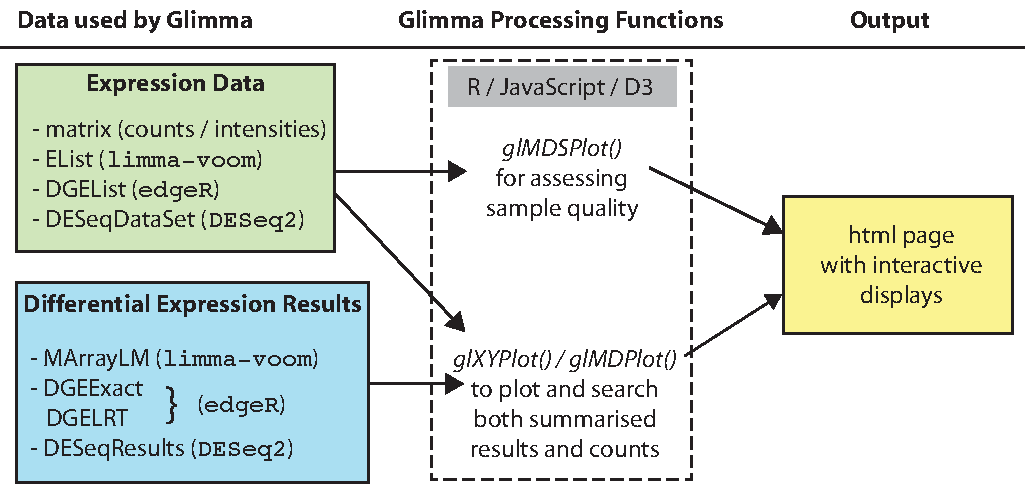
\includegraphics[width=0.65\linewidth]{GlimmaWorkFlow.pdf}}
  \caption{Overview of workflow showing the input and output types for Glimma.}
  \label{fig:overview}
\end{figure}

The main dataset used in this vignette is taken from an RNA-seq experiment examining lymphoma cell-lines in mice with alterations to the Smchd1 gene \cite{Smchd1}. The data is available for 4 wildtype samples and 3 samples with null levels of Smchd1. The count data is available within Glimma and is stored as a {\sf DGEList} object that is native to edgeR. In our analysis, we begin by removing lowly expressed genes and by performing TMM-normalisation \cite{tmm}.

\begin{Schunk}
\begin{Sinput}
> set.seed(20161000)
> options(digits=2)
> library(Glimma)
> library(limma)
> library(edgeR)
> data(lymphomaRNAseq)
> rnaseq <- lymphomaRNAseq
> rnaseq <- rnaseq[rowSums(cpm(rnaseq)>1)>=3,]
> rnaseq <- calcNormFactors(rnaseq)
\end{Sinput}
\end{Schunk}

\begin{figure}[!ht]
  \centerline{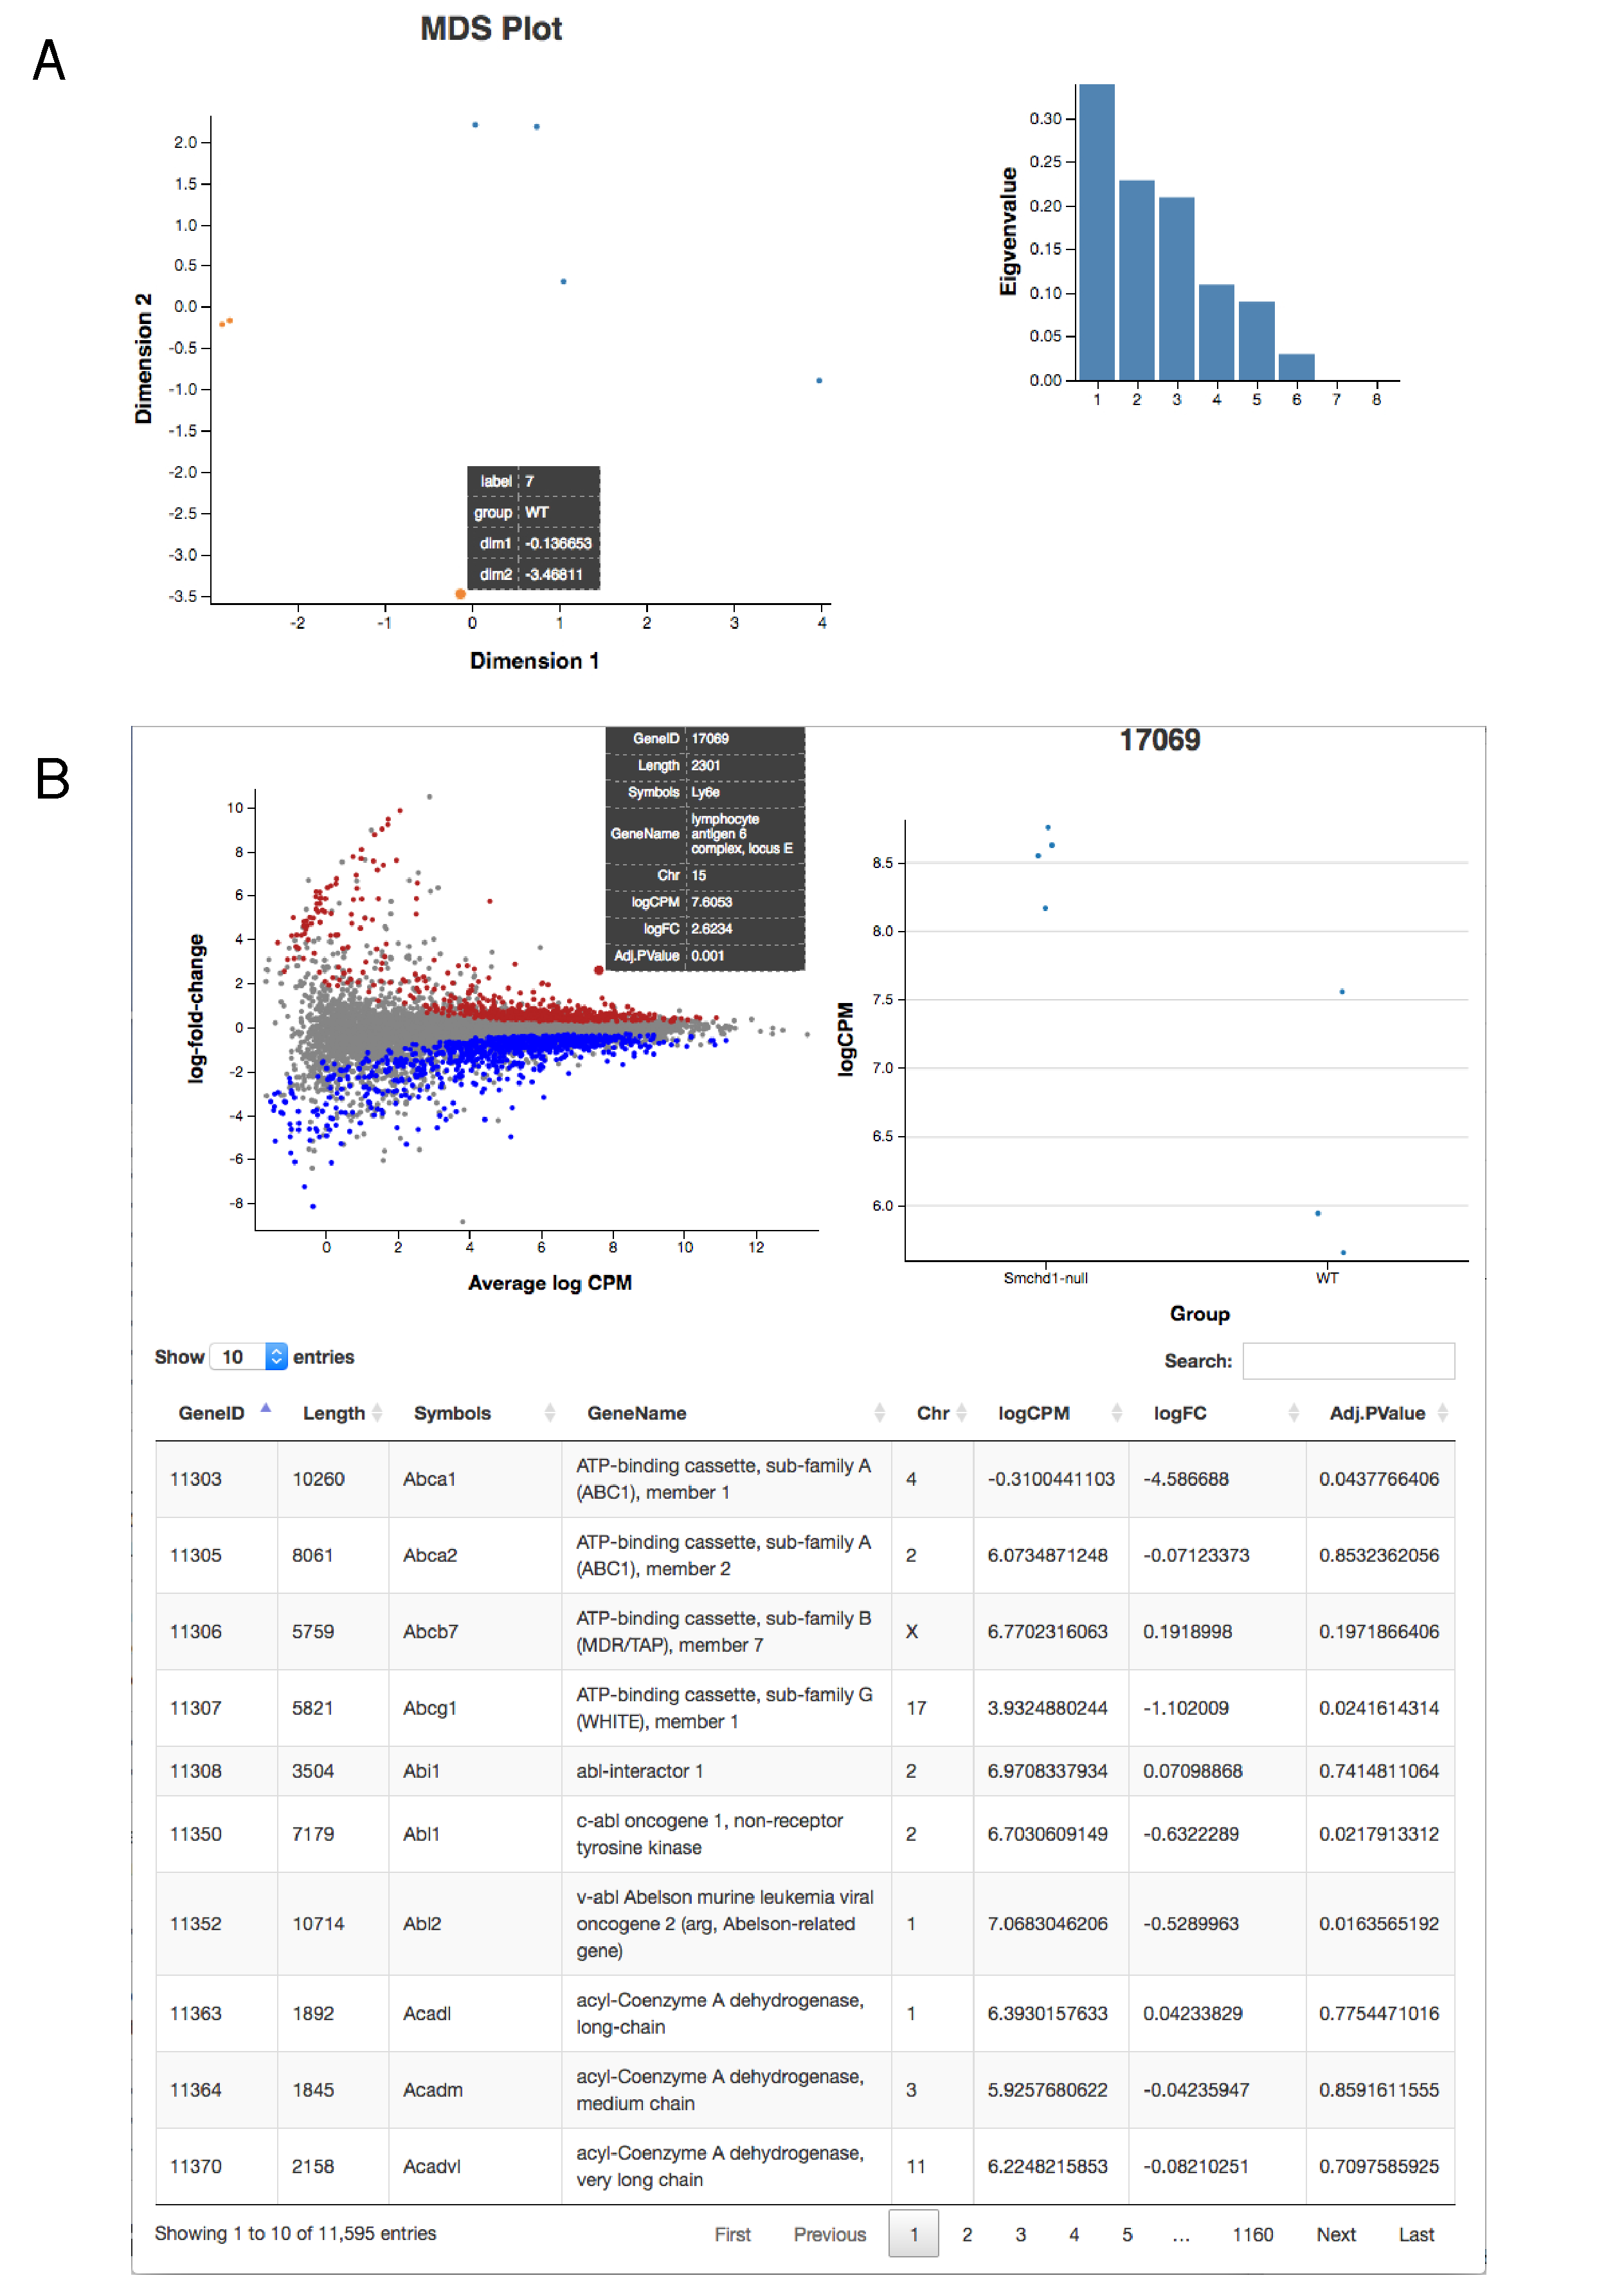
\includegraphics[width=0.7\linewidth]{quickstart.pdf}}
  \caption{A. Interactive MDS plot where the dimensions displayed in the MDS plot (left) can be changed by clicking on the associated bars in the barplot (right). B. Interactive MD plot where gene-wise logFCs are plotted against mean expression values (top left). The expression of individual samples are displayed (top right) by selecting an associated gene within the MD plot. A table of gene-wise information is displayed in the table (bottom), where genes and keywords can be searched specifically using the Search-bar.}
  \label{fig:quickstart}
\end{figure}

Using the \Rfun{glMDSPlot} functon, an interactive MDS plot can be created to examine the clustering of samples in an unsupervised fashion. Distances in the plot are used to represent similarities and dissimilarities between samples. Glimma's MDS plot allows users to interactively browse through different dimensions of the plot (Figure~\ref{fig:quickstart}A). Note that {\sf {\bf rnaseq}} is an {\sf DGEList} object.
\begin{Schunk}
\begin{Sinput}
> groups <- rnaseq$samples$group
> groups
\end{Sinput}
\begin{Soutput}
[1] Smchd1-null Smchd1-null Smchd1-null Smchd1-null WT          WT          WT         
Levels: WT Smchd1-null
\end{Soutput}
\begin{Sinput}
> glMDSPlot(rnaseq, groups=groups)
\end{Sinput}
\end{Schunk}

A limma-style analysis is carried out using voom with quality weights \cite{voom, voomqwts}, testing for the differential expression of genes between Smchd1-null and wildtype samples. For simplicity the rest of this article mostly uses limma objects to demonstrate the usage of Glimma, but Glimma works just as well on output from edgeR and DESeq2, where examples are shown explicitly in Sections~\ref{sec:appendix}. Using an adjusted p-value cutoff of 5\%, 882 genes are detected as down-regulated in the Smchd1-null group relative to wildtypes, and 634 genes as up-regulated.
\begin{Schunk}
\begin{Sinput}
> design <- model.matrix(~groups)
> colnames(design) <- c("WT", "Smchd1null.vs.WT")
> vm <- voomWithQualityWeights(rnaseq, design=design)
> fit <- lmFit(vm, design=design)
> fit <- eBayes(fit)
> dt <- decideTests(fit)
> summary(dt)
\end{Sinput}
\begin{Soutput}
      WT Smchd1null.vs.WT
-1   128              882
0    629            10079
1  10838              634
\end{Soutput}
\end{Schunk}

The results of the analysis can be examined more thoroughly through the use of Glimma's interactive MD plot which shows gene-wise log$_2$-fold changes (logFCs) plotted against average expression values and associate these to sample-specific expression values. This allows users to see summarised results from all the genes as a whole whilst being able to scrutinise the expression of individual genes at the same time. To do this, Glimma's \Rfun{glMDPlot} function is used, where significantly up- and down-regulated genes can be highlighted in red and blue respectively (Figure~\ref{fig:quickstart}B). Note that {\sf {\bf fit}} is an {\sf MArrayLM} object and {\sf {\bf dt}} is a {\sf TestResults} object.
\begin{Schunk}
\begin{Sinput}
> glMDPlot(fit, status=dt, counts=rnaseq$counts, groups=groups)
\end{Sinput}
\end{Schunk}

For more flexibility, the \Rfun{glXYPlot} allows one to plot any two vectors of equal length against each other and associate these with sample-specific expression. Here the logFC is plotted against the log-odds to create a volcano plot. As in the MD plot, genes that are differentially expressed (DE) have been highlighted. {\em It is important that genes have the same ordering in the vectors and in their expression values!}
\begin{Schunk}
\begin{Sinput}
> glXYPlot(x=fit$coef[,2], y=fit$lod[,2], status=dt[,2], counts=rnaseq$counts, groups=groups,
+   xlab="log2foldchange", ylab="logodds", anno=rnaseq$genes)
\end{Sinput}
\end{Schunk}


\section{Output settings}
All interactive plots are automatically saved as html files in a ``glimma-plots" folder that is created in the current working directory. The \Rarg{path} and \Rarg{folder} for which files are saved to can be specified within each of the Glimma functions. By default MDS plots are saved as ``MDS-Plot.html", MD plots as "MD-Plot.html", and XY plots "XY-Plot.html". Alternate file names can be specified using the \Rarg{html} argument. As each plot is created and saved, a html page is also launched automatically in your default web browser; \Rarg{launch} can be set to {\sf FALSE} if this is not desired.
%For the remainder of this article, \Rarg{launch} is set to {\sf FALSE} and file names are specified to avoid over-writing existing plots although specification of either arguments is unessential.



\section{Multi-dimensional scaling plots}
Interactive MDS plots can be created on expression data in the form of a numerical matrix or {\sf DGEList} object. Raw counts in an {\sf DGEList} are automatically converted by \Rfun{glMDSPlot} into logCPM values using normalisation factors within. For an equivalent plot using an expression matrix, counts need to be manually converted to logCPM values. Note that the {\sf cpm} function here takes into account the normalisation factors stored within the DGEList object when calculating logCPM values.
\begin{Schunk}
\begin{Sinput}
> lcpm <- cpm(rnaseq, log=TRUE, normalized.lib.sizes=TRUE)
> glMDSPlot(lcpm, groups=groups)
\end{Sinput}
\end{Schunk}

The output contains two key components. On the left is an MDS plot showing two consecutive dimensions plotted against each other with each sample represented by a point in the plot. The distance between two samples reflect the {\it leading logFC} or typical logFC for the genes separating the samples. For more information on MDS plots, see {\sf ?limma::plotMDS}. By default the top 500 genes are used to calculate distances and can be specified otherwise using the \Rarg{top} argument.

On the right, a barplot is displayed representing the proportion of variation in the data that is explained by the dimensions or eigenvectors in the MDS plot. The first, left-most bar is associated with the dimensions 1 and 2, explaining the largest proportion of variation. The second bar is associated with dimensions 2 and 3; the third bar is for dimensions 3 and 4, and so on. The dimensions that are displayed in the MDS plot can be changed by clicking on the associated bar in the barplot.

Hovering your cursor over each of the points in the MDS plot brings up information on that sample. Sample labels and group labels can be changed using the \Rarg{labels} and \Rarg{groups} arguments, where different colored points are associated with each unique group label. Typically \Rarg{groups} would be a vector specifying the main condition by which samples are separated, but for more complex experimental designs a dataframe can also be used to represent multiple categorical variables. By specifying a dataframe to the \Rarg{groups} argument, the example below shows how samples can be either colored by the {\sf groups} variable or by their sequencing {\sf lane} (Figure~\ref{fig:mdsgroups}).
\begin{Schunk}
\begin{Sinput}
> groups2 <- as.data.frame(cbind(groups=as.character(groups), lane=c(rep(4,6),3)))
> groups2
\end{Sinput}
\begin{Soutput}
       groups lane
1 Smchd1-null    4
2 Smchd1-null    4
3 Smchd1-null    4
4 Smchd1-null    4
5          WT    4
6          WT    4
7          WT    3
\end{Soutput}
\begin{Sinput}
> glMDSPlot(lcpm, groups=groups2)
\end{Sinput}
\end{Schunk}
\begin{figure}[!ht]
  \centerline{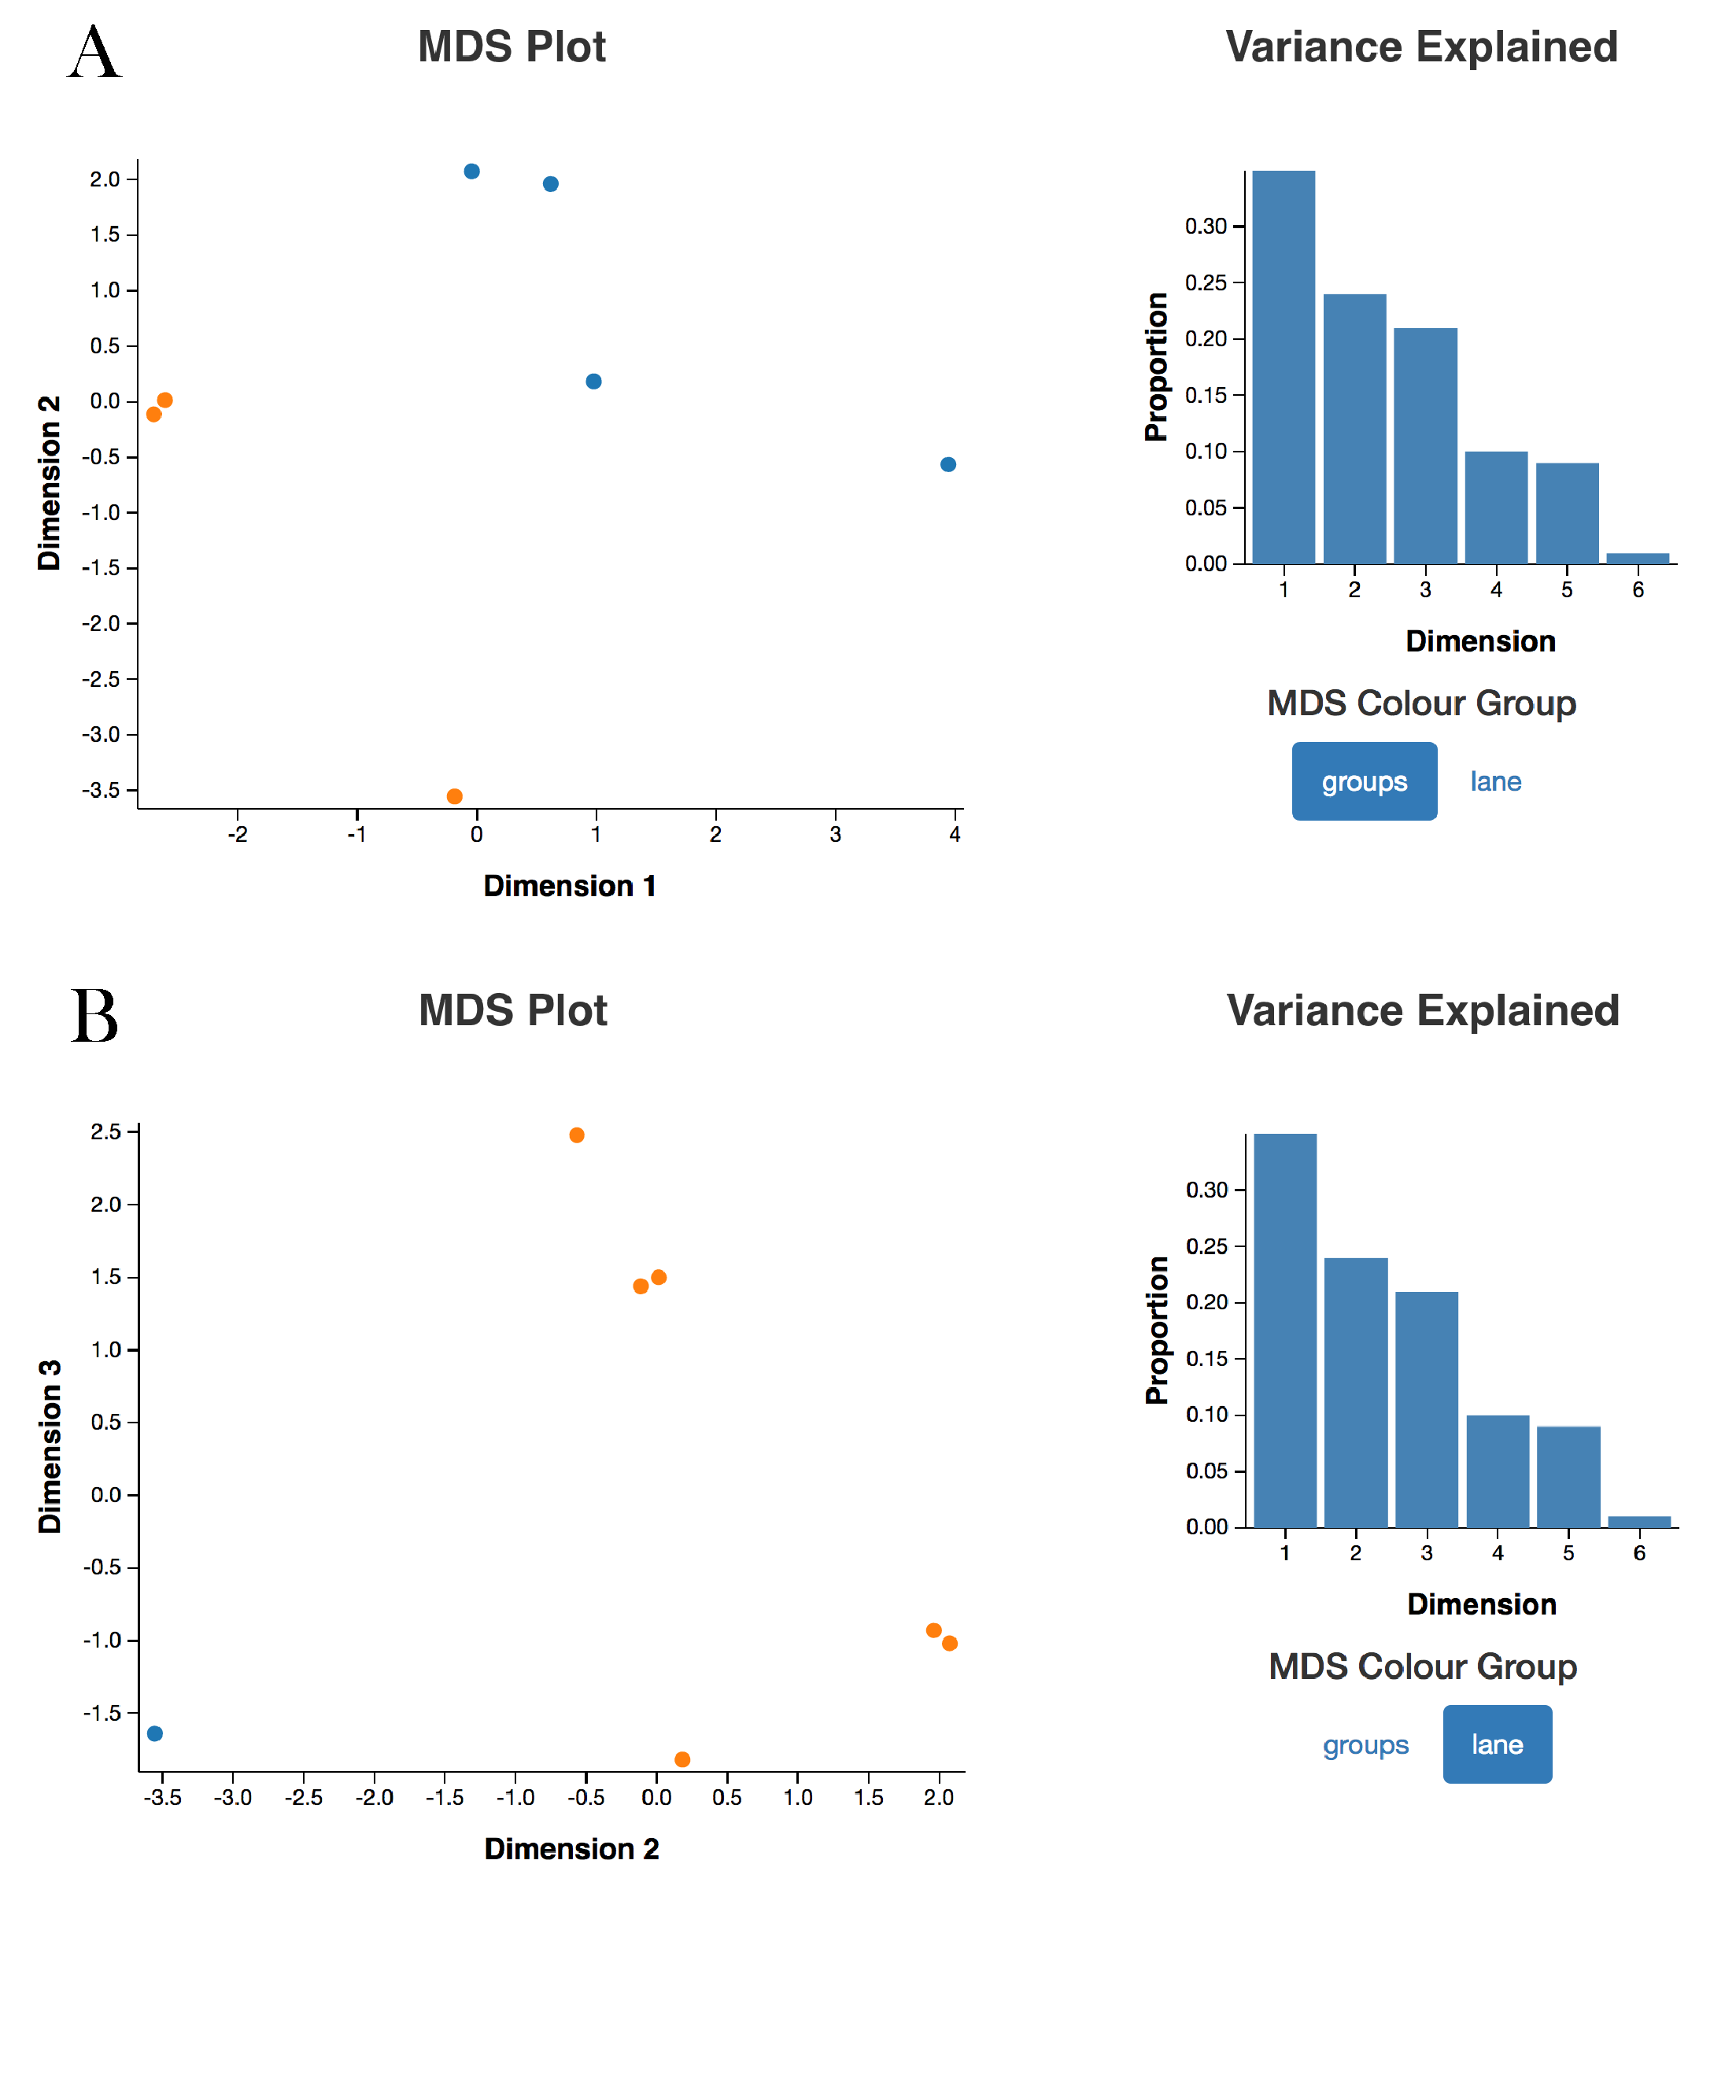
\includegraphics[width=0.7\linewidth]{MDSgroups.pdf}}
  \caption{MDS plots showing A. dimensions 1 and 2 and coloring of samples by group (or genotype) and B. dimensions 2 and 3 and coloring of samples by sequencing lane.}
  \label{fig:mdsgroups}
\end{figure}



\section{Mean-difference plots}

Interactive MD plots contain three key components, as shown in Figure~\ref{fig:quickstart}B and Figure~\ref{fig:layout}. The three components interact with each other showing multiple aspects of the data in the one display. The first and most essential component is the plot of gene-wise summarised statistics which takes the top-left position of the html page. Here, gene-wise logFCs are plotted against gene-wise average log$_2$-counts-per-million (logCPM) values where each point represents a single gene. Hovering your cursor over this main plot interacts with the plot in the top-right position which shows the expression (logCPM) of each sample for individual genes.

\begin{figure}[!ht]
  \centerline{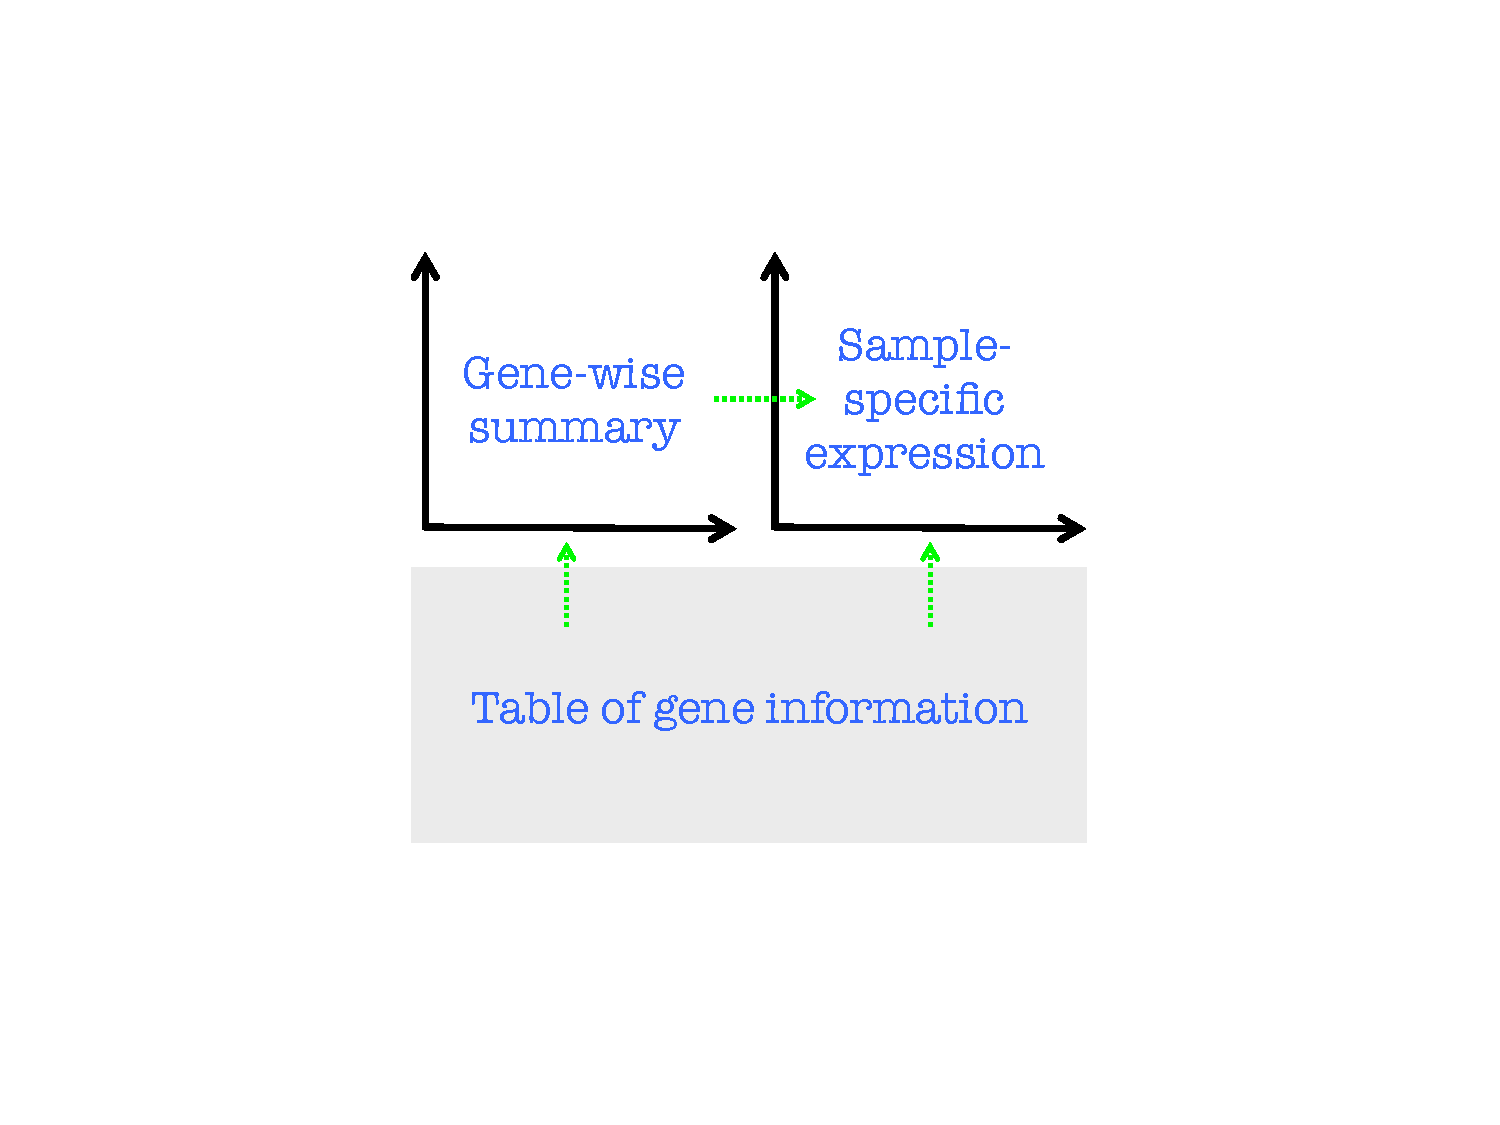
\includegraphics[width=0.4\linewidth]{Glimma_plotlayout.pdf}}
  \caption{Layout of MD plots, showing the three key components and how they interact with each other -- the direction of interaction is represented by green arrows.}
  \label{fig:layout}
\end{figure}

The MD plot is useful for exploring which genes have unusually large absolute logFC values and which of those are also highly expressed across all samples. However, such a plot does not show how much variation there is in the expression of individual samples or whether any of those samples are potential outliers. Instead these aspects can be seen in the plot of sample-specific expression. The interaction between these two plots allows users to interrogate the data more throughly by connecting gene expression information from pre-summarisation and pre-analysis to post-summarisation and post-analysis.

A table of associated gene information is positioned under the plots. This allows users to either simply scroll through a list of all the genes to look for any that is of interest, or hone into specific genes or groups of genes using  the Search-bar above the table. Clicking on a gene (or row) in the table interacts with both of the plots simultaneously -- the selected gene is highlighted in the main plot and sample-specific expression is displayed. The table can be omitted by setting \Rarg{table} to {\sf FALSE}.

Another handy function within the table is that each attribute, or column, within the table can be ordered in an increasing or decreasing fashion. By default, all genes are listed in ascending order of the variable in the first column of the table. Clicking on the name of an attribute would change the ordering the table so that it is in ascending (as indicated by a violet ``up'' arrow) or descending (as indicated by a violet ``down'' arrow) order of that attribute. This is useful for viewing the top significant genes by raw or adjusted p-value, or seeing which genes are most up- or down-regulated in terms of logFC. The ordering can be applied even on a reduced table, for example by limiting the table to down-regulated genes using the Search-bar and then ordering genes by adjusted p-value (Figure~\ref{fig:MDcoloranno}).

When working with an MArrayLM object from limma, average expression and logFC values are automatically extracted, as well as any stored gene information. By default the last coefficient is used unless specifed otherwise in \Rarg{coef}. If \Rarg{counts} is left empty, sample-specific expression is not shown and only the main plot and table will be displayed.

\begin{Schunk}
\begin{Sinput}
> glMDPlot(fit)
\end{Sinput}
\end{Schunk}

When it is used, \Rarg{counts} should be raw counts and have the same number and ordering of genes as the main argument \Rarg{x}. The function automatically transforms the counts into logCPM values. If raw counts are not used, or such a transformation is not desired then \Rarg{transform} can be set to {\sf FALSE}.

Sample-specific expression is sorted into separate groups using the \Rarg{groups} argument and colored by \Rarg{sample.cols} -- both of which are vectors matching in length and order to the samples associated with the columns in \Rarg{counts}. For most cases, \Rarg{groups} will be a character- or factor-type vector separating samples into different conditions. However, \Rarg{groups} can also be a numerical vector associated with a covariate of interest.

To demonstrate some of these options, let's say that RNA was extracted from mice of varying ages in months and create a sample-specific expression plot on raw counts versus age. The {\it real} groups are distinguished by color here (red for Smchd1-null and green for wildtype), and labels for both axes have been changed accordingly using \Rarg{side.xlab} and \Rarg{side.ylab}.

\begin{Schunk}
\begin{Sinput}
> groups.age <- runif(ncol(rnaseq), min=3, max=12)
> groups.age
\end{Sinput}
\begin{Soutput}
[1] 10.9 11.2  8.9  7.6 10.4  9.5  6.8
\end{Soutput}
\begin{Sinput}
> sample.cols <- c("limegreen", "orangered")[groups]
> sample.cols
\end{Sinput}
\begin{Soutput}
[1] "orangered" "orangered" "orangered" "orangered" "limegreen" "limegreen" "limegreen"
\end{Soutput}
\begin{Sinput}
> glMDPlot(fit, counts=rnaseq$counts, groups=groups.age, transform=FALSE,
+   sample.cols=sample.cols, side.ylab="Raw counts", side.xlab="Age (in months)")
\end{Sinput}
\end{Schunk}

\begin{figure}[!ht]
  \centerline{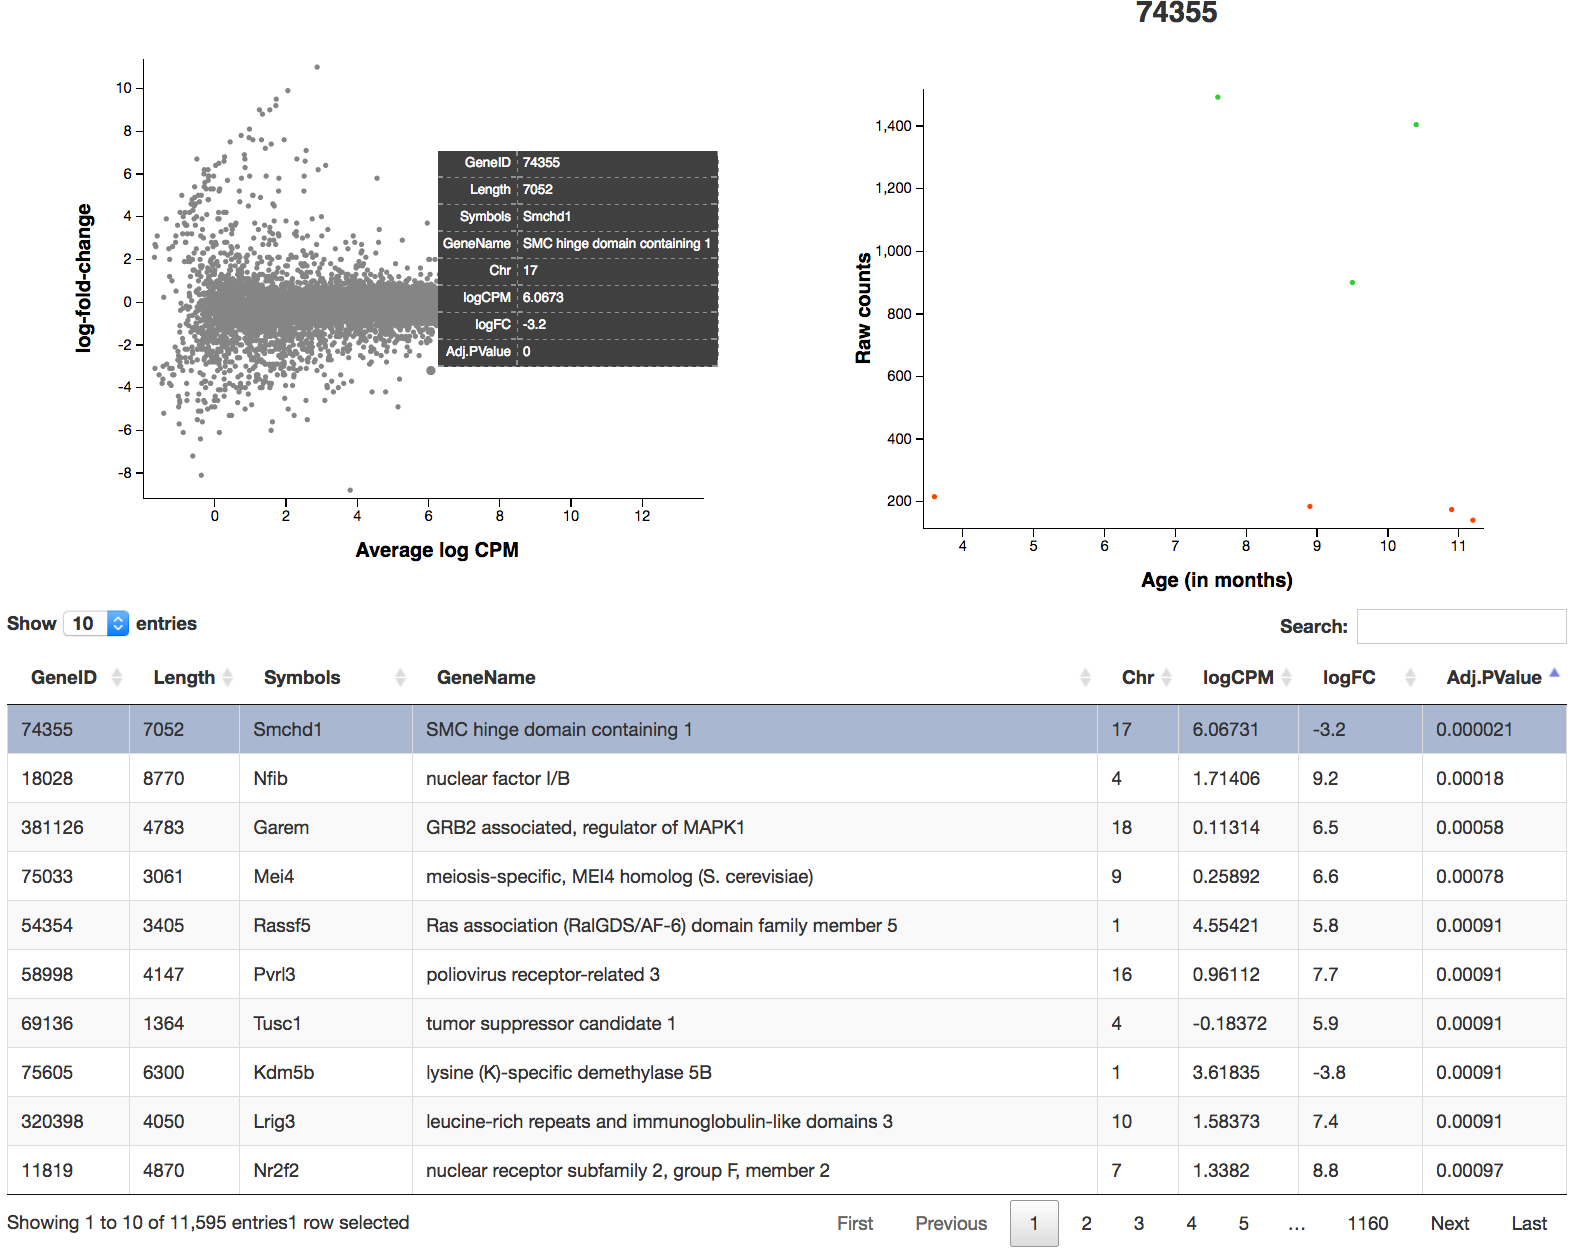
\includegraphics[width=0.7\linewidth]{MDplot_samplesasage.png}}
  \caption{MD plot, samples as age.}
  \label{fig:mdsamples}
\end{figure}

Other arguments to consider for the plot of sample-specific expression include \Rarg{id.column} for the column of gene information that is extracted for the plot's main title, \Rarg{samples} for sample labels, the amount of \Rarg{jitter} applied to points in the plot so that they don't overlap (does not apply when \Rarg{groups} is numerical), \Rarg{side.log} to plot expression on the log-scale (by default this is set to {\sf FALSE}), and \Rarg{side.gridstep} to set intervals along which horizontal grid lines are drawn (the default setting is at 0.5).

For the main plot, genes can be highlighted using the \Rarg{status} argument which contains numeric values of -1 to represent down-regulated genes (colored in blue), 0 for no differential expression (colored in grey), and 1 for up-regulated genes (colored in red). These values can be specified within a numeric vector that is of the same length and ordering of genes in \Rarg{x}. Alternatively, if a matrix is supplied with number of rows matching the number of genes, the column specified by \Rarg{coef} will be used. The colors for highlighting genes can be changed using \Rarg{cols}.

If extra gene annotation exists, this can inserted into the table using \Rarg{anno}. This would combine and display both the annotation from the MArrayLM object and from \Rarg{anno}, where \Rarg{anno} is a dataframe with the same ordering and number of genes as in \Rarg{x}. A subset of the columns displayed in the table can be specified using \Rarg{display.columns}.
\begin{Schunk}
\begin{Sinput}
> ID <- paste(fit$genes$Symbols, fit$genes$GeneID)
> DE <- c("downregulated", "notDE", "upregulated")[as.factor(dt[,2])]
> anno <- as.data.frame(cbind(ID, DE))
> head(anno)
\end{Sinput}
\begin{Soutput}
           ID            DE
1 Abca1 11303 downregulated
2 Abca2 11305         notDE
3 Abcb7 11306         notDE
4 Abcg1 11307 downregulated
5  Abi1 11308         notDE
6  Abl1 11350 downregulated
\end{Soutput}
\begin{Sinput}
> glMDPlot(fit, status=dt, counts=rnaseq$counts, groups=groups,
+   cols=c("dodgerblue", "seashell2", "maroon1"), sample.cols=sample.cols, side.gridstep=0.01,
+   anno=anno, display.columns=c("ID", "GeneName", "DE"), id.column="ID")
\end{Sinput}
\end{Schunk}

\begin{figure}[!ht]
  \centerline{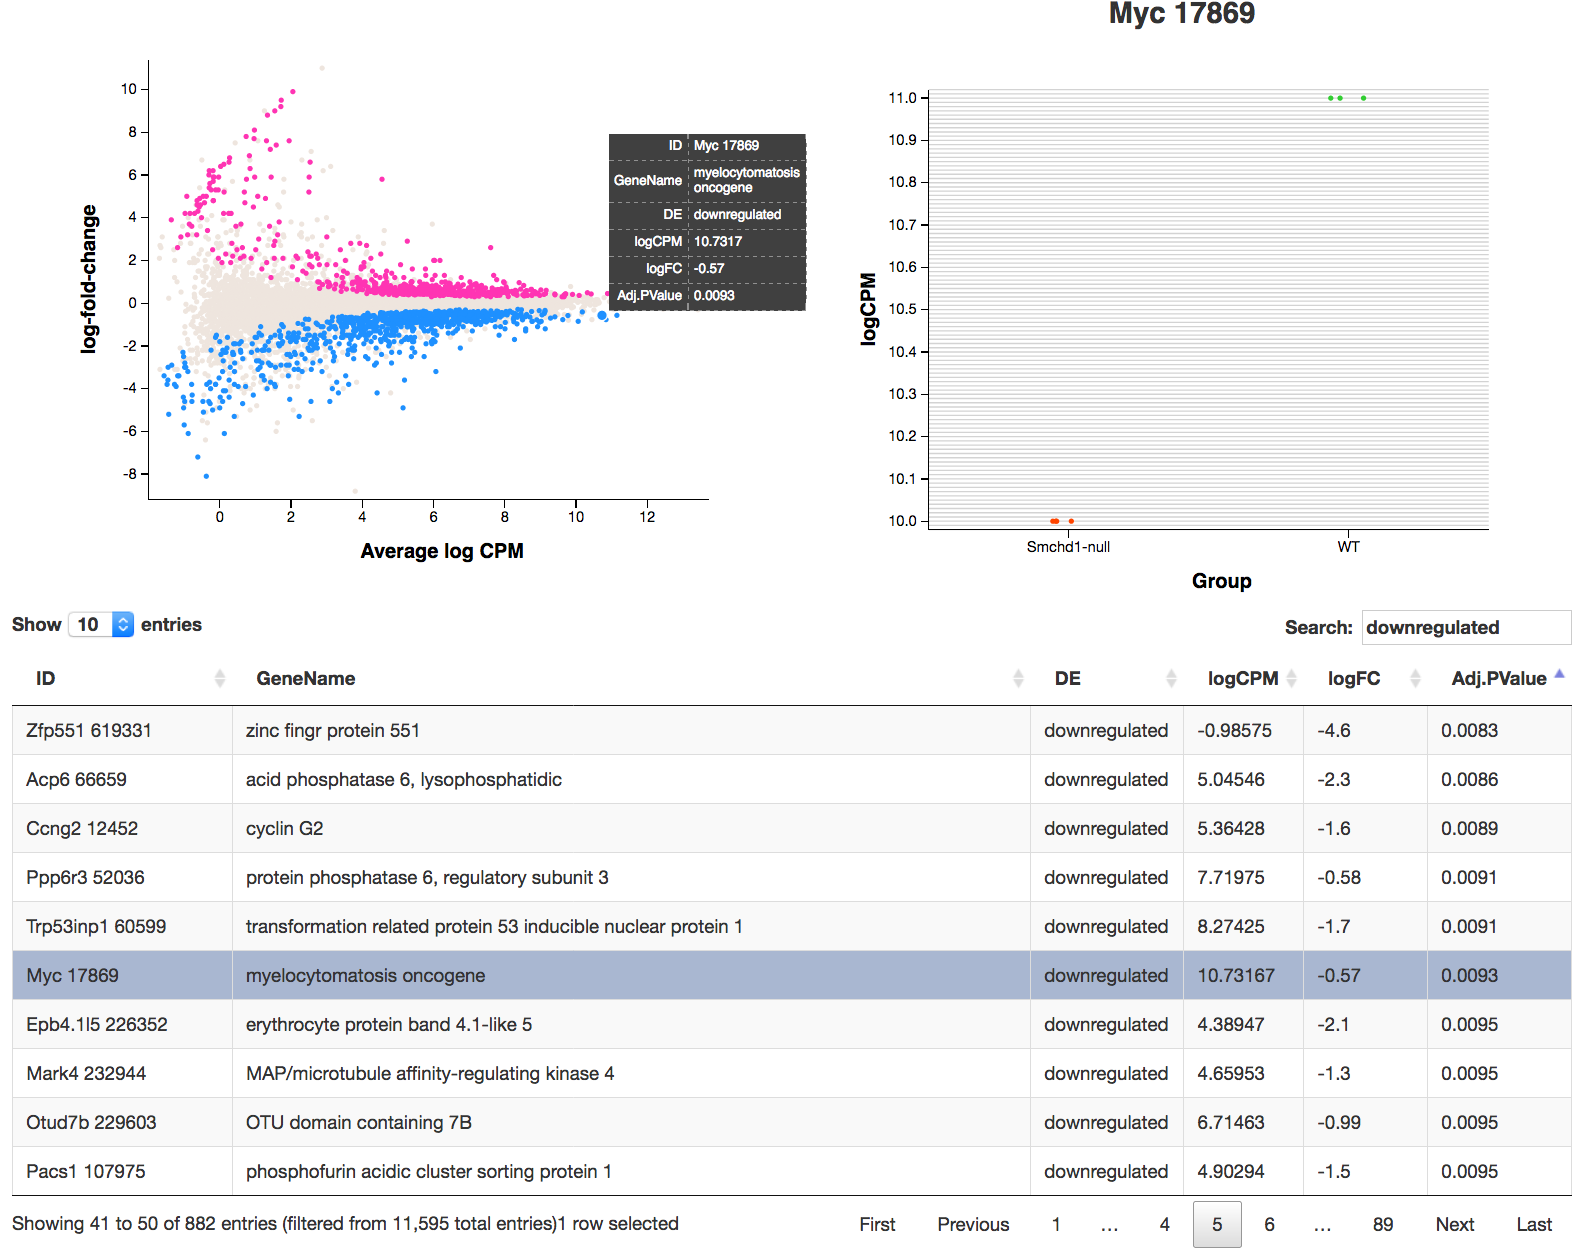
\includegraphics[width=0.7\linewidth]{MDplot_anno_myc.png}}
  \caption{Myc!!!! Interactive MD plot where up-regulated genes are colored in magenta, down-regulated genes are colored in dodger-blue, and non-DE genes are in pale-turquoise. The table of gene information is reduced to only those which are ``downregulated" using the Search-bar, and then ordered from smallest to largest adjusted p-value by clicking on the associated column label. This reveals that the Smchd1 gene is the most significantly down-regulated gene between the two groups, with Smchd1-null samples (colored in red) having lower expression of Smchd1 than samples in the wildtype (WT) group (colored in green).}
  \label{fig:MDcoloranno}
\end{figure}

Note that adjusted p-values are automatically calculated and included into the output. By default, adjusted p-values are calculated using the Benjamini and Hochberg method \cite{bh} on the raw p-values stored within the MArrayLM object. Other multiple-testing correction methods can be specified to the \Rarg{p.adj.method} argument -- see available methods within function {\sf p.adjust}.

When analysing RNA-seq data with edgeR, the R code within this section can be simply replaced by a {\sf DGEExact} or {\sf DGELRT} object produced from edgeR's exact tests and likelihood ratio tests where an {\sf MArrayLM} object was used; the same goes for {\sf DESeqDataSet} objects produced by DESeq2 analyses. Like with an {\sf MArrayLM} object, logFC values, average expression values and raw p-values (that are then corrected for multiple testing) are automatically extracted. However, gene information is not automatically extracted for DESeq2, but it is for edgeR. Subsection~\ref{sec:sec:mdedgeret}, ~\ref{sec:sec:mdedgerlrt} and ~\ref{sec:sec:mddeseq2} contains R code that produces equivalent MD plots using output from edgeR and DESeq2.



\section{XY plots}

Glimma's XY plots have the same layout as MD plots (Figure~\ref{fig:layout}) but can be used to display any gene-wise summary statistic against any other gene-wise summary statistic as the main plot. The MD plot is essentially the XY plot with the x-component specified as average logCPM values and the y-component specified as logFC values.
Since the XY plot is for general usage it works with basic R objects such as vectors, matrices and dataframes, rather than MArrayLM, DGEExact, DGELRT or DESeqDataSet objects where gene information or raw p-values could otherwise be automatically extracted. The two main arguments in \Rfun{glXYPlot} are \Rarg{x} and \Rarg{y}, both of which are numerical vectors of equal length. To create a volcano plot, we specify \Rarg{x} as the logFC between Smchd1-null versus wildtype, and \Rarg{y} as the log-odds that the gene is DE.
\begin{Schunk}
\begin{Sinput}
> glXYPlot(x=fit$coef[,2], y=fit$lod[,2])
\end{Sinput}
\end{Schunk}

Since no other information is given to the function, genes are automatically assigned gene identifiers (GeneID) and labels remain as `x' and `y'. The labels can be specified as something more meaningful, such as `logFC' and `logodds' using the arguments \Rarg{xlab} and \Rarg{ylab}, and a dataframe of gene annotation can be added using \Rarg{anno}. Like MD plots, the real advantage to XY plots are it's ability to display sample-specific expression alongside the main gene-wise summary plot using arguments \Rarg{counts} and \Rarg{groups}.

\begin{Schunk}
\begin{Sinput}
> glXYPlot(x=fit$coef[,2], y=fit$lod[,2], xlab="logFC", ylab="logodds",
+   anno=anno, counts=rnaseq$counts, groups=groups,
+   status=dt[,2], cols=c("deepskyblue", "seashell3", "firebrick1"), id.column="ID",
+   sample.cols=sample.cols)
\end{Sinput}
\end{Schunk}

\begin{figure}[!ht]
  \centerline{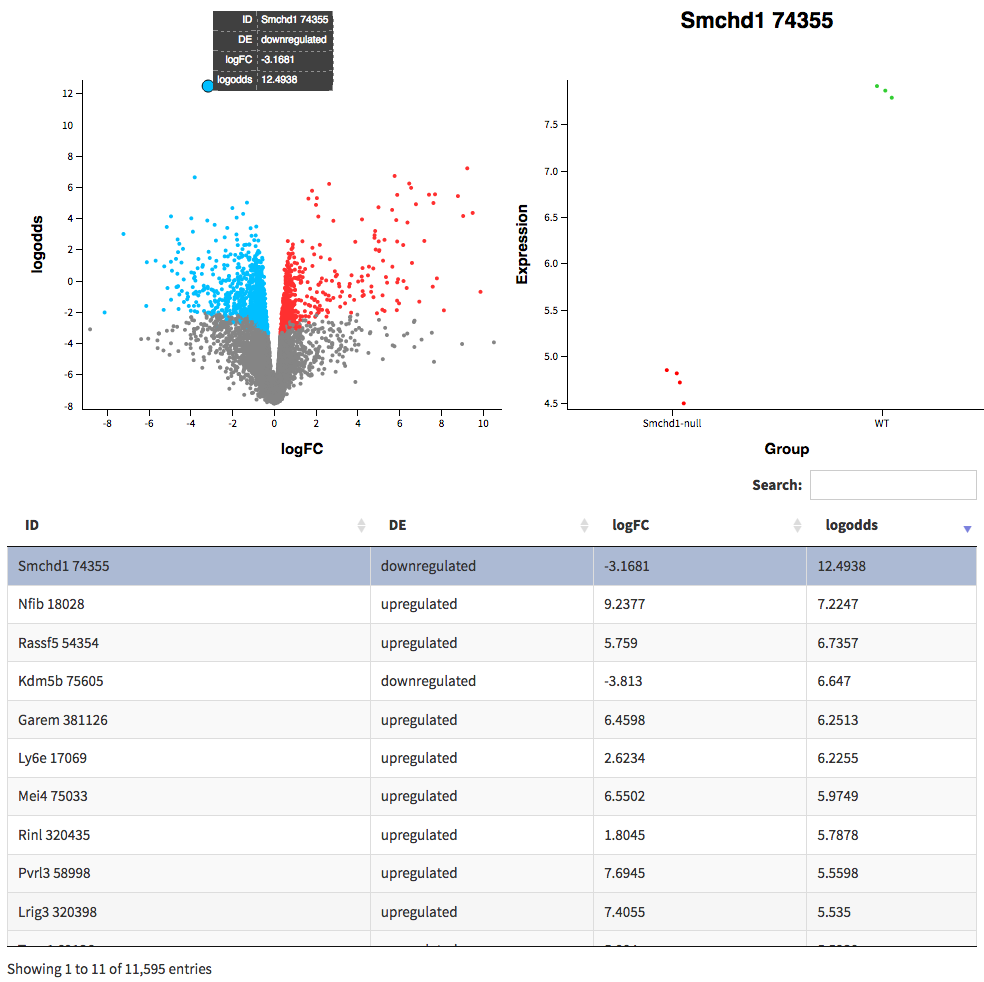
\includegraphics[width=0.7\linewidth]{XYvolcano.png}}
  \caption{XY volcano plot.}
  \label{fig:volcano}
\end{figure}

Other arguments in XY plot are analogous to those that are in the MD plot. In brief, \Rarg{status} and \Rarg{cols} are used to highlight DE genes in the main plot; \Rarg{display.columns} specifies the columns that are display within the table; in the plot of sample-specific expression, \Rarg{samples} and \Rarg{sample.cols} labels and colors points that have \Rarg{jitter} applied to avoid overlapping, and where \Rarg{id.column} is used as the main title label.

The XY plot allows users to come up with an unlimited number of plotting combinations between any two gene-wise statistcs and relate these to sample-specific expression.

\section{Microarray data}

Although Glimma was developed with RNA-sequencing data analyses in mind and designed to interacted specifically with the limma, edgeR and DESeq2, it be can just as easily applied to microarray data especially when the data is processed with limma.

Explain this dataset. Data has already been packaged into an RData object with gene information included to the EListRaw object, and a targets file with sample information.


\begin{Schunk}
\begin{Sinput}
> data(arraydata)
> arrays <- arraydata$arrays
> targets <- arraydata$targets
> arrays <- neqc(arrays)